\section{Chuyên Bắc Ninh, Bắc Ninh, lần 1, Năm 2026}
%\begin{name}
%  {Thầy Dương Tấn Đạt}
%  {Đề thi thử TN, Chuyên Bắc Ninh, Bắc Ninh, lần 1, Năm 2026}
%\end{name}

\Opensolutionfile{ans}[ans/ans-23-26-2-BacNinh-ChuyenBacNinh-L1]
\setcounter{ex}{0}
\caulc

\begin{ex}%[TT-BacNinh-ChuyenBacNinh-lan1]%[Dương Tấn Đạt, 26-2-DuAnDeTHPT2025-2026]%[1D7H2-1]
	Cho hàm số $y = \dfrac{2x - 1}{x + 1}$. Giá trị $f'(3)$ là
	\choice
	{$\dfrac{4}{5}$}
	{\True $\dfrac{3}{16}$}
	{$\dfrac{2}{9}$}
	{$\dfrac{1}{6}$}
	\loigiai{
		Ta có $y = \dfrac{2x - 1}{x + 1} \Rightarrow f'(x) = \dfrac{3}{(x + 1)^2}$.
		Khi đó $f'(3) = \dfrac{3}{(3 + 1)^2} = \dfrac{3}{16}$.
	}
\end{ex}

\begin{ex}%[TT-BacNinh-ChuyenBacNinh-lan1]%[Dương Tấn Đạt, 26-2-DuAnDeTHPT2025-2026]%[2H2N2-1]
	\immini{
		Cho hình lập phương $ABCD.A'B'C'D'$. Vectơ nào dưới đây bằng $\vec{AD}$?
		\choice
		{$\overrightarrow{BC'}$}
		{$\overrightarrow{DC}$}
		{\True $\overrightarrow{B'C'}$}
		{$\overrightarrow{AB}$}
	}{
		\begin{tikzpicture}[scale=0.5,font=\footnotesize,line join=round,line cap=round,>=stealth]
			\path
			(0,0) coordinate (B)
			(1,0.8) coordinate (A)
			(4,0) coordinate (C)
			($(C)-(B)+(A)$) coordinate (D)
			($(A)+(90:3.5)$) coordinate (A')
			($(B)-(A)+(A')$) coordinate (B')
			($(C)-(A)+(A')$) coordinate (C')
			($(D)-(A)+(A')$) coordinate (D')
			;
			\draw (B')--(B)--(C)--(D)--(D')--(A')--(B')--(C')--(D') (C)--(C');
			\draw[dashed] (A)--(D) (A')--(A)--(B);
			\foreach \p/\q in {A/160,B/-135,C/-45,D/0,A'/90,B'/180,C'/-20,D'/0}
			\fill[black] (\p)node[shift={(\q:3mm)}]{$\p$} circle (1.0pt);
		\end{tikzpicture}
	}
	\loigiai{
		Ta có $\vec{AD} = \vec{BC} = \vec{A'D'} = \vec{B'C'}$.
	}
\end{ex}

\begin{ex}%[TT-BacNinh-ChuyenBacNinh-lan1]%[Dương Tấn Đạt, 26-2-DuAnDeTHPT2025-2026]%[1D6H3-2]
	Tập xác định của hàm số $y = (x - 1)^{\frac{1}{6}} + \log (4 - x^2)$ là
	\choice
	{$[1;2)$}
	{$(-2;2)$}
	{$(1;2]$}
	{\True $(1;2)$}
	\loigiai{
		Điều kiện xác định: $
		\begin{cases}
			x - 1 > 0 \\
			4 - x^2 > 0
		\end{cases} \Leftrightarrow
		\begin{cases}
			x > 1 \\
			-2 < x < 2
		\end{cases} \Leftrightarrow 1 < x < 2$. \\
		Vậy tập xác định của hàm số là $\mathscr{D} = (1;2)$.
	}
\end{ex}

\begin{ex}%[TT-BacNinh-ChuyenBacNinh-lan1]%[Dương Tấn Đạt, 26-2-DuAnDeTHPT2025-2026]%[1D5H2-2]
	Khảo sát thời gian tập thể dục của một số học sinh khối $11$ thu được mẫu số liệu ghép nhóm sau:
	\begin{table}[h!]
		\centering
		\begin{tabular}{|c|c|c|c|c|c|}
			\hline
			\begin{tabular}{c}Thời gian\\(phút)
			\end{tabular}
			& $[0;20)$
			& $[20;40)$
			& $[40;60)$
			& $[60;80)$
			& $[80;100)$ \\
			\hline
			Số học sinh
			& $5$ & $9$ & $13$ & $10$ & $6$ \\
			\hline
		\end{tabular}
	\end{table}
	Trung vị mẫu số liệu trên gần số nào nhất?
	\choice
	{$41{,}23$}
	{\True $51{,}54$}
	{$40{,}55$}
	{$50{,}44$}
	\loigiai{
		Ta có: $n = 5 + 9 + 13 + 10 + 6 = 43$.
		Vị trí trung vị $\dfrac{n}{2} = 21{,}5$ nằm trong lớp $[40;60) \Rightarrow M_e = 40 + \dfrac{21{,}5 - 14}{13} \cdot 20 \approx 51{,}54$.
	}
\end{ex}

\begin{ex}%[TT-BacNinh-ChuyenBacNinh-lan1]%[Dương Tấn Đạt, 26-2-DuAnDeTHPT2025-2026]%[1D7H2-3]
	Cho hàm số $y = -x^3 + 3x^2 + 9x - 1$. Hệ số góc lớn nhất của tiếp tuyến với đồ thị hàm số là
	\choice
	{$9$}
	{\True $12$}
	{$6$}
	{$8$}
	\loigiai{
		Hệ số góc của tiếp tuyến với đồ thị hàm số tại điểm $A(x_A, y_A)$ là $k = f'(x_A)$.\\
		Ta có: $y' = -3x^2 + 6x + 9 = -3(x - 1)^2 + 12 \leq 12, \forall x \in \mathbb{R}$.\\
		Do đó hệ số góc lớn nhất của tiếp tuyến với đồ thị hàm số là $12$, đạt tại $x = 1$.
	}
\end{ex}

\begin{ex}%[TT-BacNinh-ChuyenBacNinh-lan1]%[Dương Tấn Đạt, 26-2-DuAnDeTHPT2025-2026]%[1D3H1-3]
	Giá trị của giới hạn $\lim \left( \sqrt[3]{n^3 - 2n^2} - n \right)$ bằng
	\choice
	{$\dfrac{1}{3}$}
	{\True $-\dfrac{2}{3}$}
	{$1$}
	{$0$}
	\loigiai{
		Ta có:
		\allowdisplaybreaks
		\begin{eqnarray*}
			\lim \left( \sqrt[3]{n^3 - 2n^2} - n \right) &=& \lim \dfrac{n^3 - 2n^2 - n^3}{\sqrt[3]{(n^3 - 2n^2)^2} + n \sqrt[3]{n^3 - 2n^2} + n^2} \\
			&=& \lim \dfrac{-2n^2}{\sqrt[3]{(n^3 - 2n^2)^2} + n \sqrt[3]{n^3 - 2n^2} + n^2} \\
			&=& \lim \dfrac{-2}{\sqrt[3]{\left( 1 - \dfrac{2}{n} \right)^2} + n \sqrt[3]{1 - \dfrac{2}{n}} + 1} = -\dfrac{2}{3}.
		\end{eqnarray*}
	}
\end{ex}

\begin{ex}%[TT-BacNinh-ChuyenBacNinh-lan1]%[Dương Tấn Đạt, 26-2-DuAnDeTHPT2025-2026]%[1H4H4-6]
	Cho hai hình bình hành $ABCD$ và $ABEF$ không cùng nằm trong một mặt phẳng. Gọi $O_1, O_2$ lần lượt là tâm của $ABCD, ABEF$. $M$ là trung điểm của $CD$. Chọn khẳng định sai trong các khẳng định sau.
	\choice
	{\True $MO_2$ cắt $(BEC)$}
	{$O_1O_2$ song song với $(AFD)$}
	{$O_1O_2$ song song với $(BEC)$}
	{$O_1O_2$ song song với $(EFM)$}
	
	\loigiai{
		\begin{center}
			\begin{tikzpicture}[scale=1, font=\footnotesize, line join=round, line cap=round, >=stealth]
				% 1. Định nghĩa tọa độ các điểm cơ bản
				\path
				(0,0) coordinate (A)
				(5,0) coordinate (D)
				(1.5,1.5) coordinate (B)
				(6.5,1.5) coordinate (C)
				(0.5,3.5) coordinate (F)
				(2,5) coordinate (E)
				;
				% 2. Xác định tâm O_1, O_2 và trung điểm M
				\coordinate (O_1) at (intersection of A--C and B--D);
				\coordinate (O_2) at (intersection of A--E and B--F);
				\coordinate (M) at ($(C)!0.5!(D)$);
				% 3. Vẽ các cạnh khuất (dashed)
				\draw[dashed] (B)--(C) (B)--(A) (B)--(E) (B)--(F) (B)--(D) (O_1)--(O_2) (M)--(O_2) (O_1)--(M);
				% 4. Vẽ các cạnh thấy
				\draw (A)--(D) (D)--(C) (C)--(A) (A)--(F) (F)--(E) (E)--(C) (F)--(D) (A)--(E);
				% 5. Dán nhãn và vẽ điểm
				\foreach \p/\q in {A/180, F/180, O_2/180, B/180, D/0, C/0, M/0, E/90, O_1/-90}
				\fill[black] (\p) circle (1.0pt) ($(\p)+(\q:3mm)$) node{$\p$};
			\end{tikzpicture}
		\end{center}
		Dễ thấy $O_1 O_2$ là đường trung bình của tam giác $ACE \Rightarrow O_1 O_2 \parallel CE \Rightarrow O_1 O_2 \parallel (BEC)$.\\
		Tương tự, $O_1 O_2 \parallel DF \Rightarrow O_1 O_2 \parallel (ADF)$.\\
		Từ đó suy ra $O_1 O_2 \parallel (CDFE)$ hay $O_1 O_2 \parallel (MEF)$.\\
		Ta có $
		\begin{cases} O_1 O_2 \parallel CE \\ O_1 M \parallel BC
		\end{cases} \Rightarrow (O_1 O_2 M) \parallel (BCE)$, do đó $MO_2$ nằm trong mặt phẳng song song với $(BEC)$ nên không thể cắt $(BEC)$.\\
		Như vậy khẳng định $MO_2$ cắt $(BEC)$ là khẳng định sai.
	}
\end{ex}

\begin{ex}%[TT-BacNinh-ChuyenBacNinh-lan1]%[Dương Tấn Đạt, 26-2-DuAnDeTHPT2025-2026]%[1D1N4-6]
	Tập giá trị của hàm số $y = \cot x$ là
	\choice
	{$(-1;1)$}
	{$[-1;1]$}
	{\True $\mathbb{R}$}
	{$(-\infty;0)$}
	\loigiai{
		Tập giá trị của hàm số $y = \cot x$ là $\mathbb{R}$.
	}
\end{ex}

\begin{ex}%[TT-BacNinh-ChuyenBacNinh-lan1]%[Dương Tấn Đạt, 26-2-DuAnDeTHPT2025-2026]%[2H2N1-1]
	Cho tứ diện $ABCD$. Gọi $G$ là trọng tâm của tam giác $ABC$. Phát biểu nào sau đây là sai?
	\choice
	{$\vec{DA} + \vec{DB} + \vec{DC} = 3\vec{DG}$}
	{$\vec{GD} - \vec{GA} = \vec{AD}$}
	{$\vec{GA} + \vec{GB} + \vec{GC} = \vec{0}$}
	{\True $\vec{GA} + \vec{GB} + \vec{GC} + \vec{GD} = \vec{0}$}
	\loigiai{
		\immini{
			Vì $G$ là trọng tâm tam giác $ABC$ nên ta có $\vec{GA} + \vec{GB} + \vec{GC} = \vec{0}$ \\
			$\Rightarrow \vec{GA} + \vec{GB} + \vec{GC} + \vec{GD} = \vec{GD} \neq \vec{0}$.
		}{
			\begin{tikzpicture}[line join=round, line cap=round, >=stealth, scale=1.2, font=\footnotesize]
				% Định nghĩa các đỉnh tứ diện
				\path
				(1.5, 3) coordinate (D)
				(0.0, 1.2) coordinate (A)
				(1.6, 0.0) coordinate (B)
				(4.0, 1.2) coordinate (C)
				;
				\coordinate (M) at ($(A)!0.5!(B)$);
				\coordinate (G) at ($(C)!2/3!(M)$);
				
				\draw (D)--(A) (D)--(B) (D)--(C) (A)--(B) (B)--(C);
				\draw[dashed] (A)--(C) (D)--(G) (A)--(G) (B)--(G) (C)--(G);
				\foreach \p/\q in {D/90, A/180, B/-90, C/0, G/-45}
				\fill[black] (\p) circle (1.0pt) node[shift={(\q:3mm)}]{$\p$};
			\end{tikzpicture}
		}
	}
\end{ex}

\begin{ex}%[TT-BacNinh-ChuyenBacNinh-lan1]%[Dương Tấn Đạt, 26-2-DuAnDeTHPT2025-2026]%[1D3H1-5]
	Tìm số hạng tổng quát của cấp số nhân lùi vô hạn khi có tổng bằng $3$ và công bội bằng $\dfrac{2}{3}$.
	\choice
	{\True $\left( \dfrac{2}{3} \right)^{n - 1}$}
	{$\left( \dfrac{2}{3} \right)^n$}
	{$\left( \dfrac{2}{3} \right)^{n + 1}$}
	{$\left( \dfrac{2}{3} \right)^{n + 1}$}
	\loigiai{
		Ta có $S = \dfrac{u_1}{1 - q} \Leftrightarrow 3 = \dfrac{u_1}{1 - \dfrac{2}{3}} \Leftrightarrow u_1 = 1$.
		Cấp số nhân có $
		\begin{cases}
			u_1 = 1 \\
			q = \dfrac{2}{3}
		\end{cases} \Rightarrow u_n = u_1 q^{n-1} = 1 \cdot \left( \dfrac{2}{3} \right)^{n - 1} = \left( \dfrac{2}{3} \right)^{n - 1}$.
	}
\end{ex}

\begin{ex}%[TT-BacNinh-ChuyenBacNinh-lan1]%[Dương Tấn Đạt, 26-2-DuAnDeTHPT2025-2026]%[1H4H4-6]
	\immini{
		Cho lăng trụ $ABCD.A'B'C'D'$ có hai đáy là các hình bình hành. Các điểm $M,N,P$ lần lượt là trung điểm của cạnh $AD, BC, CC'$ (tham khảo hình vẽ). Xét các khẳng định sau:
		\begin{enumerate}[a)]
			\item Mặt phẳng $(MNP)$ cắt $A'D'$.
			\item Mặt phẳng $(MNP)$ cắt $DD'$ tại trung điểm của $DD'$.
			\item Mặt phẳng $(MNP)$ song song với mặt phẳng $(ABC'D')$.
		\end{enumerate}
	}{
		\begin{tikzpicture}[scale=0.5, font=\footnotesize, line join=round, line cap=round, >=stealth]
			\coordinate (A) at (0,0);
			\coordinate (D) at (4.5,0);
			\coordinate (B) at (-1.5,-1.5);
			\coordinate (C) at ($(B)+(D)-(A)$);
			\coordinate (A') at (1.5,3.5);
			\coordinate (B') at ($(B)+(A')-(A)$);
			\coordinate (C') at ($(C)+(A')-(A)$);
			\coordinate (D') at ($(D)+(A')-(A)$);
			
			\coordinate (M) at ($(A)!0.5!(D)$);
			\coordinate (N) at ($(B)!0.5!(C)$);
			\coordinate (P) at ($(C)!0.5!(C')$);
			
			\draw[dashed] (A)--(D) (A)--(B) (A)--(A') (M)--(N) (M)--(P);
			\draw (B)--(C)--(D)--(D')--(C')--(B')--cycle;
			\draw (A')--(D') (A')--(B') (C)--(C') (N)--(P);
			
			\foreach \p/\q in {A/135, A'/135, B'/180, B/-135, C/-45, D/0, C'/0, D'/45, P/0, M/135, N/-90}
			\fill[black] (\p) circle (1.0pt) node[shift={(\q:3mm)}]{$\p$};
		\end{tikzpicture}
	}
	Trong các khẳng định trên, số khẳng định đúng là:
	\choice
	{$0$}
	{$1$}
	{\True $3$}
	{$2$}
	\loigiai{
		\begin{center}
			\begin{tikzpicture}[scale=1, font=\footnotesize, line join=round, line cap=round, >=stealth]
				\path
				(0,0) coordinate (A)
				(4.5,0) coordinate (D)
				(-1.5,-1.5) coordinate (B)
				($(B)+(D)-(A)$) coordinate (C)
				(1.5,3.5) coordinate (A')
				($(B)+(A')-(A)$) coordinate (B')
				($(C)+(A')-(A)$) coordinate (C')
				($(D)+(A')-(A)$) coordinate (D')
				
				($(A)!0.5!(D)$) coordinate (M)
				($(B)!0.5!(C)$) coordinate (N)
				($(C)!0.5!(C')$) coordinate (P)
				($(D)!0.5!(D')$) coordinate (Q)
				;
				
				\draw[dashed] (A)--(D) (A)--(B) (A)--(A') (M)--(N) (M)--(P) (M)--(Q);
				\draw (B)--(C)--(D)--(D')--(C')--(B')--cycle;
				\draw (A')--(D') (A')--(B') (C)--(C');
				\draw (N)--(P)--(Q);
				
				\foreach \p/\q in {B'/180, B/-135, A/135, A'/135, D/0, C'/0, P/0, Q/0, D'/45, M/135, N/-90, C/-45}
				\fill[black] (\p) circle (1.0pt) node[shift={(\q:3mm)}]{$\p$};
			\end{tikzpicture}
		\end{center}
		\begin{enumerate}[a)]
			\item Do $M, N$ lần lượt là trung điểm của $AD, BC$ nên $MN \parallel AB \parallel CD$. Tuy nhiên $MN$ không song song với $AD$ (và cũng không song song với $A'D'$). Gọi $Q$ là giao điểm giữa mặt phẳng $(MNP)$ với $DD'$ ($Q \in DD'$). Ta có $(MNP) \cap (ADD'A') = MQ$. Vì $MQ$ và $A'D'$ cùng nằm trong mặt phẳng $(ADD'A')$ và không song song với nhau nên chúng cắt nhau. Khẳng định "mặt phẳng $(MNP)$ cắt $A'D'$" là khẳng định đúng.
			\item Ta có: $MN \parallel CD \Rightarrow CD \parallel (MNQP) \Rightarrow CD \parallel QP$. Mà $P$ là trung điểm $CC'$ nên $Q$ là trung điểm $DD'$. Do đó khẳng định này đúng.
			\item Ta có: $MP$ là đường trung bình của tam giác $(BC'C) \Rightarrow MP \parallel BC'$.
			Lại có $MN \parallel AB$, do đó $(MNQP) \parallel (ABC'D')$, khẳng định này đúng.
		\end{enumerate}
		Vậy có $3$ khẳng định đúng.
	}
\end{ex}

\begin{ex}%[TT-BacNinh-ChuyenBacNinh-lan1]%[Dương Tấn Đạt, 26-2-DuAnDeTHPT2025-2026]%[2D1N1-2]
	\immini{
		Cho hàm số đa thức bậc ba $y = ax^3 + bx^2 + cx + d$ $(a \neq 0)$ có đồ thị như hình vẽ.
		Hàm số đã cho nghịch biến trên khoảng nào dưới đây?
		\choice
		{$(-2;0)$}
		{$(0;+\infty)$}
		{$(-1;1)$}
		{\True $(1;+\infty)$}
	}{
		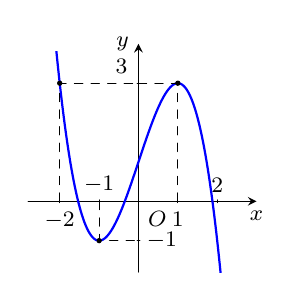
\begin{tikzpicture}[font=\footnotesize, line join=round, line cap=round, >=stealth, scale=0.5]
			\draw[->] (-2.8,0)--(3,0) node[below] {$x$};
			\draw[->] (0,-1.8)--(0,4) node[left] {$y$};
			\draw (0,0) node [below right] {$O$};
			
			\draw[thin] (-2,1pt)--(-2,-1pt) node[below] {$-2$};
			\draw[thin] (-1,1pt)--(-1,-1pt) node[above] {$-1$};
			\draw[thin] (1,1pt)--(1,-1pt)   node[below] {$1$};
			\draw[thin] (2,1pt)--(2,-1pt)   node[above] {$2$};
			
			\draw[thin] (1pt,3)--(-1pt,3)   node[above left] {$3$};
			\draw[thin] (1pt,-1)--(-1pt,-1) node[right] {$-1$};
			\begin{scope}
				\clip (-2.8,-1.8) rectangle (2.8,3.8);
				\draw[blue, thick, samples=200, domain=-2.3:2.3, smooth, variable=\x]
				plot (\x, {-(\x)^3 + 3*(\x) + 1});
			\end{scope}
			
			% Đường dashed cực đại tại (1, 3)
			\draw[dashed] (1,0) -- (1,3) -- (0,3);
			% Đường dashed cực tiểu tại (-1, -1)
			\draw[dashed] (-1,0) -- (-1,-1) -- (0,-1);
			\draw[dashed] (-2,0)--(-2,3)--(0,3);
			% Chấm tại các điểm
			\filldraw[black] (1,3) circle (1.5pt);
			\filldraw[black] (-1,-1) circle (1.5pt);
			\filldraw[black] (-2,3) circle (1.5pt);
		\end{tikzpicture}
	}
	\loigiai{
		Hàm số đã cho nghịch biến trên khoảng $(1;+\infty)$.
	}
\end{ex}

\cauds

\begin{ex}%[TT-BacNinh-ChuyenBacNinh-lan1]%[Dương Tấn Đạt, 26-2-DuAnDeTHPT2025-2026]%[2D1V5-3]
	\immini{
		Cho hàm số $y = f(x)$ có đạo hàm trên $\mathbb{R}$ và $f'(x)$ là hàm số bậc ba có đồ thị là đường cong trong hình vẽ.
		\choiceTF
		{Đồ thị hàm số $g(x) = f(x) - \dfrac{1}{2} x^2 + x + 2025$ cắt đường thẳng $y = m$ tại bốn điểm phân biệt khi và chỉ khi $g(-1) < m < \min\{g(-3);g(1)\}$}
		{\True Đồ thị hàm số $h(x) = \dfrac{2x+1}{f'(x)}$ có $3$ đường tiệm cận}
		{Hàm số $y = f(x)$ đồng biến trên khoảng $(0;+\infty)$}
		{Hàm số $y = f(x)$ có hai điểm cực trị}
	}{
		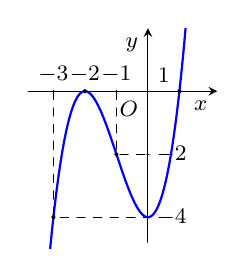
\begin{tikzpicture}[font=\footnotesize, line join=round, line cap=round, >=stealth,scale=0.4]
			\draw[->] (-3.8,0)--(2.2,0) node[below left] {$x$};
			\draw[->] (0,-4.8)--(0,2) node[below left] {$y$};
			\draw (0,0) node[below left] {$O$};
			% Mốc trục x thủ công
			\draw[thin] (-3,1pt)--(-3,-1pt) node[above] {$-3$};
			\draw[thin] (-2,1pt)--(-2,-1pt) node[above] {$-2$};
			\draw[thin] (-1,1pt)--(-1,-1pt) node[above] {$-1$};
			\draw[thin] (1,1pt)--(1,-1pt)   node[above left] {$1$};
			
			% Mốc trục y thủ công
			\draw[thin] (1pt,-2)--(-1pt,-2) node[right] {$-2$};
			\draw[thin] (1pt,-4)--(-1pt,-4) node[right] {$-4$};
			\begin{scope}
				\clip (-3.8,-5) rectangle (2,2);
				% f'(x) = (x + 2)^2*(x - 1)
				\draw[blue, thick, samples=200, domain=-3.5:1.5, smooth, variable=\x]
				plot (\x, {(\x + 2)^2*(\x - 1)});
			\end{scope}
			
			% Dashed: điểm (-3, -4)
			\draw[dashed] (-3,0)--(-3,-4)--(0,-4);
			% Dashed: điểm (-1, -2)
			\draw[dashed] (-1,0)--(-1,-2)--(0,-2);
			% Dashed: điểm (1, 0) — chỉ chấm
			% Dashed: điểm (-2, 0) — trên trục x
			
			% Chấm các điểm đặc biệt
			\filldraw[black] (-3,-4) circle (1.5pt);
			\filldraw[black] (-2,0)  circle (1.5pt);
			\filldraw[black] (-1,-2) circle (1.5pt);
			\filldraw[black] (1,0)   circle (1.5pt);
		\end{tikzpicture}
	}
	\loigiai{
		\begin{itemchoice}
			\itemch \textbf{Sai.}
			\begin{center}
				\resizebox{0.45\textwidth}{!}{
					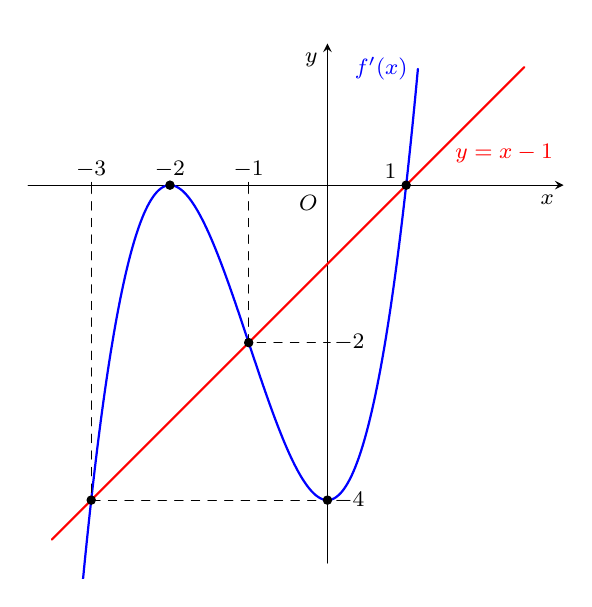
\begin{tikzpicture}[font=\footnotesize, line join=round, line cap=round, >=stealth]
						\draw[->] (-3.8,0)--(3,0) node[below left] {$x$};
						\draw[->] (0,-4.8)--(0,1.8) node[below left] {$y$};
						\draw (0,0) node[below left] {$O$};
						% Mốc trục x thủ công
						\draw[thin] (-3,1pt)--(-3,-1pt) node[above] {$-3$};
						\draw[thin] (-2,1pt)--(-2,-1pt) node[above] {$-2$};
						\draw[thin] (-1,1pt)--(-1,-1pt) node[above] {$-1$};
						\draw[thin] (1,1pt)--(1,-1pt)   node[above left] {$1$};
						% Mốc trục y thủ công
						\draw[thin] (1pt,-2)--(-1pt,-2) node[right] {$-2$};
						\draw[thin] (1pt,-4)--(-1pt,-4) node[right] {$-4$};
						\draw (1.5,0.4) node[right] {$\textcolor{red}{y = x - 1}$};
						
						\begin{scope}
							\clip (-3.8,-5) rectangle (3,2);
							% f'(x) = (x + 2)^2*(x - 1)
							\draw[blue, thick, samples=200, domain=-3.5:1.15, smooth, variable=\x]
							plot (\x, {(\x + 2)^2*(\x - 1)}) node[left] {$\textcolor{blue}{f'(x)}$};
							% Đường thẳng y = x - 1
							\draw[red, thick, domain=-3.5:2.5, variable=\x]
							plot (\x, {\x - 1});
						\end{scope}
						
						% Dashed: điểm (-3, -4)
						\draw[dashed] (-3,0)--(-3,-4)--(0,-4);
						% Dashed: điểm (-1, -2)
						\draw[dashed] (-1,0)--(-1,-2)--(0,-2);
						% Dashed: điểm (1, 0) — chỉ chấm
						% Dashed: điểm (-2, 0) — trên trục x
						
						% Chấm các điểm đặc biệt
						\filldraw[black] (-3,-4) circle (1.5pt);
						\filldraw[black] (-2,0)  circle (1.5pt);
						\filldraw[black] (-1,-2) circle (1.5pt);
						\filldraw[black] (1,0)   circle (1.5pt);
						\filldraw[black] (0,-4)  circle (1.5pt);
					\end{tikzpicture}
				}
			\end{center}
			Ta có: $g(x) = f(x) - \dfrac{1}{2}x^2 + x + 2025 \Rightarrow g'(x) = f'(x) - x + 1 = f'(x) - (x-1)$.
			Xét đồ thị hàm số $f'(x)$ và đồ thị hàm số $y = x - 1$, ta thấy
			$$f'(x) - (x-1) = 0 \Leftrightarrow \left[
			\begin{aligned} &x = -3 \\ &x = -1 \\ &x = 1
			\end{aligned}\right.$$
			Từ đó, ta có bảng biến thiên như sau:
			\begin{center}
				
\begin{tikzpicture}
					\tkzTabInit[lgt=2, espcl=2]
					{$x$ / 0.8, $g'(x)$ / 0.8, $g(x)$ / 2}
					{$-\infty$, $-3$, $-1$, $1$, $+\infty$}
					\tkzTabLine{, -, 0, +, 0, -, 0, +}
					\tkzTabVar{+/$+\infty$, -/$g(-3)$, +/$g(-1)$, -/$g(1)$, +/$+\infty$}
				\end{tikzpicture}
			\end{center}
			Dựa vào bảng biến thiên, ta thấy để phương trình $g(x) = m$ có $4$ nghiệm phân biệt thì $\max\{g(-3);\ g(1)\} < m < g(-1)$.
			\itemch \textbf{Đúng.}
			Xét hàm số $h(x) = \dfrac{2x + 1}{f'(x)}$. \\
			Ta có $f'(x) = 0 \Leftrightarrow \left[
			\begin{aligned} &x = 1\\&x = -2
			\end{aligned}\right.$, mà $
			\begin{cases} 2(1) + 1 = 3 \neq 0 \\ 2(-2) + 1 = -3 \neq 0
			\end{cases}$, do đó đồ thị hàm số $h(x) = \dfrac{2x+1}{f'(x)}$ có $2$ đường tiệm cận đứng tại $x = 1$ và $x = -2$. \\
			Mặt khác, do bậc mẫu lớn hơn bậc tử nên $\lim_{x \to -\infty} h(x) = \lim_{x \to +\infty} h(x) = 0$, do đó đồ thị hàm số $h(x)$ có $1$ đường tiệm cận ngang $y = 0$. \\
			Vậy đồ thị hàm số $h(x) = \dfrac{2x + 1}{f'(x)}$ có $3$ đường tiệm cận.
			\itemch \textbf{Sai.} Trên khoảng $(0;+\infty)$, ta thấy $
			\begin{cases}
				f'(x) < 0, x \in (0;1) \\
				f'(x) > 0, x \in (1;+\infty)
			\end{cases}$.\\
			Suy ra hàm số $f(x)$ nghịch biến trên khoảng $(0;1)$ và đồng biến trên khoảng $(1;+\infty)$.
			\itemch \textbf{Sai.} Dựa vào đồ thị của hàm số $f'(x)$, ta thấy $f'(x) = 0$ có $1$ nghiệm bội lẻ ($x = 1$), do đó hàm số $f(x)$ có $1$ điểm cực trị.
		\end{itemchoice}
	}
\end{ex}

\begin{ex}%[TT-BacNinh-ChuyenBacNinh-lan1]%[Dương Tấn Đạt, 26-2-DuAnDeTHPT2025-2026]%[1H8V7-3]
	Cho hình chóp tứ giác đều $S.ABCD$ có cạnh đáy bằng $a$, cạnh bên bằng $\sqrt{2}a$. Gọi $F$ là trung điểm của cạnh $SA$.
	\choiceTF
	{\True Khoảng cách từ $S$ đến mặt phẳng $(FCD)$ bằng $\dfrac{a\sqrt{10}}{5}$}
	{Độ lớn của góc giữa đường thẳng $SA$ và mặt phẳng đáy bằng $30^\circ$}
	{Thể tích của khối chóp $S.FCD$ bằng $\dfrac{a^3\sqrt{3}}{24}$}
	{\True Khoảng cách giữa $AC$ và $SB$ bằng $\dfrac{a\sqrt{6}}{4}$}
	\loigiai{
		\begin{center}
			\resizebox{0.5\textwidth}{!}{
				\begin{tikzpicture}[scale=1, font=\footnotesize, line join=round, line cap=round, >=stealth]
					\path
					(3.75, 7.0) coordinate (S)
					(0.0, 1.0) coordinate (D)
					(5.5, 1.0) coordinate (C)
					(7.5, 3.0) coordinate (B)
					(2.0, 3.0) coordinate (A)
					;
					\coordinate (O) at ($(A)!0.5!(C)$);
					\coordinate (F) at ($(S)!0.5!(A)$);
					\coordinate (I) at ($(S)!0.5!(B)$);
					
					\draw[dashed] (S)--(A)--(D) (A)--(B) (A)--(C) (B)--(D) (S)--(O);
					\draw[brown, dashed] (F)--(C) (F)--(D);
					\draw[red, dashed] (O)--(I)--(C) (A)--(I);
					
					\draw (S)--(D)--(C)--(B)--cycle (S)--(C);
					\foreach \p/\q in {S/90, A/180, B/0, C/-45, D/-135, O/-90, F/0, I/45}
					\fill[black] (\p) circle (1.0pt) node[shift={(\q:3mm)}]{$\p$};
				\end{tikzpicture}
			}
		\end{center}
		\begin{itemchoice}
			\itemch \textbf{Đúng.} Tam giác $SAC$ đều $\left(SA = SC = AC = a\sqrt{2}\right)$ có trung tuyến $FC = \dfrac{\sqrt{3}}{2} \cdot a \sqrt{2} = \dfrac{a \sqrt{6}}{2}$. \\
			Tam giác $SAD$ có $DF$ là đường trung tuyến $\Rightarrow DF = \sqrt{\dfrac{SD^2 + AD^2}{2} - \dfrac{SA^2}{4}} = a$. \\
			Tam giác $FCD$ có $CD = a,\ DF = a,\ FC = \dfrac{a\sqrt{6}}{2}$
			$$\Rightarrow S_{FCD} = \sqrt{p(p-FC)(p-CD)(p-DF)}, \text{ với } p = \dfrac{4+\sqrt{6}}{4}a$$
			$$\Rightarrow S_{FCD} = \dfrac{\sqrt{15}}{8} \cdot a^2.$$
			Lại có $V_{S.FCD} = \dfrac{1}{3} d \left( S,(FCD) \right) \cdot S_{FCD} \Rightarrow d\left( S,(FCD) \right) = \dfrac{3V_{S.FCD}}{S_{FCD}} = \dfrac{a \sqrt{10}}{5}$.
			\itemch \textbf{Sai.} $\widehat{(SA,(ABCD))} = \widehat{(SA, AO)} = \widehat{SAO}.$ \\
			Tam giác $SAO$ có $\cos\widehat{SAO} = \dfrac{AO}{SA} = \dfrac{a\sqrt{2}/2}{a\sqrt{2}} = \dfrac{1}{2} \Rightarrow \widehat{SAO} = 60^\circ$. \\
			Như vậy $\widehat{(SA,(ABCD))} = \widehat{(SA, AO)} = 60^\circ$. Khẳng định $30^\circ$ là sai.
			
			\itemch \textbf{Sai.} Gọi $O$ là tâm hình vuông $ABCD$, khi đó $SO$ là đường cao của hình chóp $S.ABCD$.
			Tam giác vuông $SAO$ có $SA = a \sqrt{2},\ AO = \dfrac{AC}{2} = \dfrac{a \sqrt{2}}{2}$ \\
			$\Rightarrow SO = \sqrt{SA^2 - AO^2} = \sqrt{\left( a \sqrt{2} \right)^2 - \left( \dfrac{a \sqrt{2}}{2} \right)^2} = \dfrac{a \sqrt{6}}{2}.$ \\
			Suy ra $V_{S.ABCD} = \dfrac{1}{3} \cdot SO \cdot S_{ABCD} = \dfrac{1}{3} \cdot SO \cdot AB^2 = \dfrac{a^3\sqrt{6}}{6}$.
			Từ đó $V_{S.FCD} = V_{A.FCD} = \dfrac{1}{2}V_{S.ACD} = \dfrac{1}{4}V_{S.ABCD} = \dfrac{a^3\sqrt{6}}{24}$.
			
			\itemch \textbf{Đúng.} Kẻ $OI \perp SB$ ($I \in SB$). Dễ thấy hình chóp $S.ABCD$ đối xứng qua mặt phẳng $(SAC)$ nên ta có $CI = IA$. \\
			Do đó tam giác $AIC$ cân tại $I \Rightarrow OI \perp AC$. Suy ra $d(AC, SB) = OI$. \\
			Xét tam giác $SOB$ có $\dfrac{1}{OI^2} = \dfrac{1}{SO^2} + \dfrac{1}{OB^2} \Rightarrow OI = \dfrac{a \sqrt{6}}{4}$ hay $d(AC, SB) = \dfrac{a \sqrt{6}}{4}$.
		\end{itemchoice}
	}
\end{ex}

\begin{ex}%[TT-BacNinh-ChuyenBacNinh-lan1]%[Dương Tấn Đạt, 26-2-DuAnDeTHPT2025-2026]%[0D0V2-7]
	Trong hộp có $45$ quả cầu có cùng kích thước và khối lượng được đánh số từ $1$ đến $45$. Lấy ngẫu nhiên $3$ quả cầu từ hộp đó. Xét tính đúng sai của các mệnh đề sau:
	\choiceTF
	{\True Số cách lấy được cả $3$ quả cầu đánh số chẵn bằng $1540$}
	{Xác suất để tích $3$ số ghi trên $3$ quả cầu là một số chia hết cho $8$ bằng $\dfrac{523}{1290}$}
	{Xác suất để tổng $3$ số ghi trên $3$ quả cầu là số lẻ bằng $\dfrac{1}{2}$}
	{\True Xác suất để tổng $3$ số ghi trên $3$ quả cầu là số chia hết cho $4$ bằng $\dfrac{323}{1290}$}
	\loigiai{
		\begin{itemchoice}
			\itemch \textbf{Đúng.} Trong $45$ quả cầu có $22$ quả cầu mang số chẵn, $23$ quả cầu mang số lẻ. Do đó số cách lấy được cả $3$ quả cầu đánh số chẵn bằng $\mathrm{C}_{22}^3 = 1540$ (cách).
			\itemch \textbf{Sai.} Ta xét các trường hợp tích $3$ số ghi trên $3$ quả cầu là số không chia hết cho $8$:
			\begin{enumerate}[\textbf{TH\arabic*:}]
				\item Ba số là ba số lẻ. Số cách lấy là $\mathrm{C}_{23}^3$ (cách).
				\item Trong ba số có $2$ số lẻ, và số chẵn còn lại không chia hết cho $8$. Có $5$ số chia hết cho $8$ ($8, 16, 24, 32, 40$) , do đó có $17$ số chẵn không chia hết cho $8$. Do đó có $\mathrm{C}_{23}^2 \cdot \mathrm{C}_{17}^1$ (cách).
				\item Trong ba số có $1$ số lẻ, và tích $2$ số chẵn còn lại không chia hết cho $8$. Khi đó, $2$ số chẵn còn lại phải có dạng $4k + 2, k \in \mathbb{N}$ (có $11$ số như vậy). Do đó có $\mathrm{C}_{23}^1 \cdot \mathrm{C}_{11}^2$ (cách).
			\end{enumerate}
			Như vậy, có $\mathrm{C}_{23}^3 + \mathrm{C}_{23}^2 \cdot \mathrm{C}_{17}^1 + \mathrm{C}_{23}^1 \cdot \mathrm{C}_{11}^2 = 7337$ cách để chọn ra $3$ số có tích không chia hết cho $8$.\\
			Số cách chọn ra $3$ số là: $\mathrm{C}_{45}^3 = 14190$ (cách).\\
			Vậy xác suất để tích $3$ số ghi trên $3$ quả cầu là một số chia hết cho $8$ bằng: $1 - \dfrac{7337}{14190} = \dfrac{6853}{14190} = \dfrac{623}{1290}$.
			\itemch \textbf{Sai.} Ta xét các trường hợp để tổng $3$ số được chọn là một số lẻ:
			\begin{enumerate}[\textbf{TH\arabic*:}]
				\item Cả ba số đều là số lẻ. Số cách chọn là $\mathrm{C}_{23}^3$ (cách chọn).
				\item Trong $3$ số có $1$ số lẻ và $2$ số chẵn. Số cách chọn là $\mathrm{C}_{23}^1 \cdot \mathrm{C}_{22}^2$ (cách chọn).
			\end{enumerate}
			Tổng số cách chọn là: $\mathrm{C}_{23}^3 + \mathrm{C}_{23}^1 \cdot \mathrm{C}_{22}^2 = 7084$ (cách chọn). \\
			Xác suất để tổng $3$ số ghi trên $3$ quả cầu là số lẻ bằng $\dfrac{7084}{\mathrm{C}_{45}^3} = \dfrac{322}{645}$.
			\itemch \textbf{Đúng.} Trong $45$ số, có $11$ số chia hết cho $4$, $12$ số chia $4$ dư $1$, $11$ số chia $4$ dư $2$ và $11$ số chia $4$ dư $3$.
			Ta xét các trường hợp để tổng $3$ số ghi trên $3$ quả cầu là số chia hết cho $4$:
			\begin{enumerate}[\textbf{TH\arabic*:}]
				\item $3$ số đều chia hết cho $4$, số cách chọn là $\mathrm{C}_{11}^3$ (cách).
				\item Có $1$ số chia hết cho $4$ và $2$ số chia $4$ dư $2$. Số cách chọn là $\mathrm{C}_{11}^1 \cdot \mathrm{C}_{11}^2$ (cách).
				\item Có $1$ số chia $4$ dư $2$, và $2$ số chia $4$ dư $1$. Số cách chọn là $\mathrm{C}_{11}^1 \cdot \mathrm{C}_{12}^2$ (cách).
				\item Có $1$ số chia $4$ dư $2$, và $2$ số chia $4$ dư $3$. Số cách chọn là $\mathrm{C}_{11}^1 \cdot \mathrm{C}_{11}^2$ (cách).
				\item Có $1$ số chia hết cho $4$, $1$ số chia $4$ dư $1$ và $1$ số chia $4$ dư $3$. Số cách chọn là $\mathrm{C}_{11}^1 \cdot \mathrm{C}_{12}^1 \cdot \mathrm{C}_{11}^1$ (cách chọn).
			\end{enumerate}
			Tổng số cách chọn là: $\mathrm{C}_{11}^3 + \mathrm{C}_{11}^1 \cdot \mathrm{C}_{11}^2 + \mathrm{C}_{11}^1 \cdot \mathrm{C}_{12}^2 + \mathrm{C}_{11}^1 \cdot \mathrm{C}_{11}^2 + \mathrm{C}_{11}^1 \cdot \mathrm{C}_{12}^1 \cdot \mathrm{C}_{11}^1 = 3553$ (cách). \\
			Xác suất để tổng $3$ số ghi trên $3$ quả cầu là số chia hết cho $4$ là: $\mathrm{P} = \dfrac{3553}{\mathrm{C}_{45}^3} = \dfrac{323}{1290}$.
		\end{itemchoice}
	}
\end{ex}

\begin{ex}%[TT-BacNinh-ChuyenBacNinh-lan1]%[Dương Tấn Đạt, 26-2-DuAnDeTHPT2025-2026]%[2D1V3-1]
	Cho hàm số $y = (9 - x^2)^\frac{1}{3} + \ln (1 - x)$.
	\choiceTF
	{Tập xác định của hàm số là khoảng $(-\infty;1)$}
	{Hàm số có đạo hàm $y' = \dfrac{1}{\sqrt[3]{(9 - x^2)^2}} - \dfrac{1}{1 - x}$}
	{\True Hàm số nghịch biến trên khoảng $(0;1)$}
	{\True Giá trị nhỏ nhất của hàm số trên đoạn $\left[ \dfrac{1}{4}; \dfrac{1}{2} \right]$ bằng $\dfrac{1}{2} \sqrt[3]{70} - \ln 2$}
	\loigiai{
		\begin{itemchoice}
			\itemch \textbf{Sai.} ĐKXĐ:
			$
			\begin{cases}
				9 - x^2 > 0 \\
				1 - x > 0
			\end{cases} \Leftrightarrow
			\begin{cases}
				-3 < x < 3 \\
				x < 1
			\end{cases} \Leftrightarrow -3 < x < 1$.
			Tập xác định của hàm số là $(-3;1)$.
			\itemch \textbf{Sai.} Với $-3 < x < 1$, ta có: $y' = -\dfrac{2x}{3\sqrt[3]{(9 - x^2)^2}} - \dfrac{1}{1 - x}$.
			\itemch \textbf{Đúng.} Với $0 < x < 1$, ta có:
			$
			\begin{cases}
				\dfrac{2x}{3\sqrt[3]{(9 - x^2)^2}} > 0 \\
				1 - x > 0
			\end{cases} \Rightarrow y' = -\dfrac{2x}{3\sqrt[3]{(9 - x^2)^2}} - \dfrac{1}{1 - x} < 0$. Do đó hàm số nghịch biến trên khoảng $(0;1)$.
			\itemch \textbf{Đúng.} Do hàm số nghịch biến trên khoảng $(0;1)$ nên
			$$\min \limits_{\left[ \frac{1}{4}; \frac{1}{2} \right]} f(x) = f \left( \dfrac{1}{2} \right) = \sqrt[3]{\dfrac{35}{4}} - \ln 2 = \dfrac{1}{2} \sqrt[3]{70} - \ln 2.$$
		\end{itemchoice}
	}
\end{ex}

\caukq

\begin{ex}%[TT-BacNinh-ChuyenBacNinh-lan1]%[Dương Tấn Đạt, 26-2-DuAnDeTHPT2025-2026]%[0H5V4-4]
	Cho hai vectơ $\vec{a}, \vec{b}$ sao cho $|\vec{a}| = \sqrt{2}, |\vec{b}| = 2$ và hai vectơ $\vec{x} = \vec{a} + \vec{b},\ \vec{y} = 2\vec{a} - \vec{b}$ vuông góc với nhau. Tính góc giữa hai véc tơ $\vec{a}$ và $\vec{b}$ (đơn vị độ).
	\shortans{$90$}
	\loigiai{
		Ta có: $\vec{x} \perp \vec{y} \Rightarrow \vec{x} \cdot \vec{y} = 0 \Leftrightarrow \left(\vec{a} + \vec{b}\right)\left(2\vec{a} - \vec{b}\right) = 0 \Leftrightarrow 2a^2 - b^2 + \vec{a}\vec{b} = 0$ \\
		$\Leftrightarrow \vec{a} \cdot \vec{b} = 2 \cdot (\sqrt{2})^2 - 2^2 = 0 \Rightarrow \vec{a} \perp \vec{b}$.
		Vậy góc giữa véc tơ $\vec{a}$ và $\vec{b}$ bằng $90^\circ$.
	}
\end{ex}

\begin{ex}%[TT-BacNinh-ChuyenBacNinh-lan1]%[Dương Tấn Đạt, 26-2-DuAnDeTHPT2025-2026]%[2D1V2-3]
	Tính tổng tất cả các giá trị nguyên của tham số $m$ để hàm số $y = \dfrac{x^2 + (m - 1)x + 3 - 2m}{x + m}$ đạt cực tiểu tại $x = -1$.
	\shortans{$2$}
	\loigiai{
		Ta có: $y = \dfrac{x^2 + (m - 1)x + 3 - 2m}{x + m} = x - 1 + \dfrac{3 - m}{x + m} \Rightarrow y' = 1 - \dfrac{3 - m}{(x + m)^2} \Rightarrow y'' = \dfrac{2(3 - m)}{(x + m)^3}.$ \\
		Để hàm số đạt cực tiểu tại $x = -1$ thì:
		$$
		\begin{cases}
			y'(-1) = 0 \\ y''(-1) > 0
		\end{cases} \Leftrightarrow
		\begin{cases}
			1 - \dfrac{3 - m}{(-1 + m)^2} = 0 \\
			\dfrac{2(3 - m)}{(-1 + m)^3} > 0
		\end{cases} \Leftrightarrow
		\begin{cases}
			\left[
			\begin{aligned} &m = -1 \\ &m = 2
			\end{aligned}\right. \\
			1 < m < 3
		\end{cases} \Rightarrow m = 2.$$
		Vậy $m = 2$ thoả mãn điều kiện.
	}
\end{ex}

\begin{ex}%[TT-BacNinh-ChuyenBacNinh-lan1]%[Dương Tấn Đạt, 26-2-DuAnDeTHPT2025-2026]%[2H2V1-4]
	Một chiếc ô tô được đặt trên mặt đáy dưới của một khung sắt dạng hình hộp chữ nhật với đáy trên là hình chữ nhật $ABCD$, mặt phẳng $(ABCD)$ song song với mặt phẳng nằm ngang. Khung sắt đó được đặt vào móc $E$ của chiếc cần cẩu sao cho các đoạn dây cáp $EA,EB,EC,ED$ bằng nhau và cùng tạo với mặt phẳng $(ABCD)$ một góc $\alpha$.
	Chiếc cần cẩu kéo khung sắt lên theo phương thẳng đứng. Biết các lực căng $\vec{F_1}, \vec{F_2}, \vec{F_3}, \vec{F_4},$ đều có cường độ là $4800$ N, trọng lượng của cả khung sắt chứa xe ô tô là $7200 \sqrt{6}$ N. Tính $\sin \alpha$ (làm tròn kết quả đến chữ số hàng phần trăm).
	\shortans{$0{,}92$}
	\loigiai{
		\begin{center}
			\resizebox{0.45\textwidth}{!}{
				\begin{tikzpicture}[scale=1, font=\footnotesize, line join=round, line cap=round, >=stealth]
					\path
					(3.5, 7.0) coordinate (E)
					(1.5, 3.0) coordinate (A)
					(7.0, 3.0) coordinate (B)
					(5.5, 1.0) coordinate (C)
					(0.0, 1.0) coordinate (D)
					;
					\coordinate (O) at ($(A)!0.5!(C)$);
					\coordinate (SF1) at ($(E)!4/5!(A)$);
					\coordinate (SF2) at ($(E)!4/5!(B)$);
					\coordinate (SF3) at ($(E)!4/5!(C)$);
					\coordinate (SF4) at ($(E)!4/5!(D)$);
					\draw[dashed] (A)--(B) (A)--(D) (A)--(C) (B)--(D);
					\draw[->, dashed, thick, blue] (E)--(A);
					\draw[->, dashed, thick, blue] (E)--(O);
					
					\draw (E)--(B) (E)--(C) (E)--(D) (B)--(C) (C)--(D);
					\draw[->, thick, blue] (E)--(B);
					\draw[->, thick, blue] (E)--(C);
					\draw[->, thick, blue] (E)--(D);
					\draw pic[draw=red, angle radius=0.6cm] {angle = C--A--E};
					\path (A) ++(18:0.8cm) node[red] {$\alpha$};
					
					\foreach \p/\q in {E/90, A/-90, B/0, C/-45, D/-135, O/-90}
					\fill[black] (\p) circle (1.0pt) node[shift={(\q:3mm)}]{$\p$};
					\node[right] at (SF1) {$\vec{F_1}$};
					\node[right] at (SF2) {$\vec{F_2}$};
					\node[right] at (SF3) {$\vec{F_3}$};
					\node[left]  at (SF4) {$\vec{F_4}$};
					\node[above right] at (O) {$\vec{P}$};
				\end{tikzpicture}
			}
		\end{center}
		Ta có: $\vec{P} = \vec{F_1} + \vec{F_2} + \vec{F_3} + \vec{F_4} = 4\vec{F_1} \cdot \sin\alpha \Rightarrow |\vec{P}| = 4|\vec{F_1}| \cdot \sin\alpha$ \\
		$\Leftrightarrow 7200\sqrt{6} = 4 \cdot 4800 \cdot \sin \alpha \Leftrightarrow \sin \alpha = \dfrac{7200\sqrt{6}}{4 \cdot 4800} \approx 0{,}92$.
	}
\end{ex}

\begin{ex}%[TT-BacNinh-ChuyenBacNinh-lan1]%[Dương Tấn Đạt, 26-2-DuAnDeTHPT2025-2026]%[1H4V3-5]
	Cho hình tứ diện $ABCD$ có tất cả các cạnh bằng $6$. Gọi $M, N$ lần lượt là trung điểm của $CA, CB$. $P$ là điểm trên cạnh $BD$ sao cho $BP = 2PD$. Gọi $(H)$ là hình giới hạn bởi giao tuyến của mặt phẳng $(MNP)$ với các mặt của tứ diện $ABCD$. Tính diện tích hình $(H)$ (kết quả làm tròn đến hàng phần trăm).
	\shortans{$8{,}93$}
	\loigiai{
		\begin{center}
			\resizebox{0.45\textwidth}{!}{
				\begin{tikzpicture}[scale=1, font=\footnotesize, line join=round, line cap=round, >=stealth]
					\path
					(0,0) coordinate (A)
					(6.5,0) coordinate (B)
					(2.5,-1.5) coordinate (C)
					(3,3.5) coordinate (D)
					;
					\coordinate (M) at ($(C)!0.5!(A)$);
					\coordinate (N) at ($(C)!0.5!(B)$);
					\coordinate (P) at ($(D)!1/3!(B)$);
					\coordinate (Q) at ($(D)!1/3!(A)$);
					
					\draw[dashed] (A)--(B) (Q)--(P) (Q)--(N);
					\draw (A)--(C) (C)--(B) (B)--(D) (D)--(A) (C)--(D);
					\draw[thick, blue] (M)--(Q) (Q)--(P) (P)--(N);
					\draw[thick, blue, dashed] (N)--(M);
					
					\foreach \p/\q in {A/180, Q/135, M/-135, B/0, P/45, N/-45, C/-90, D/90} {
						\fill[black] (\p) circle (1.0pt);
						\node[shift={(\q:3mm)}] at (\p) {$\p$};
					}
				\end{tikzpicture}
			}
		\end{center}
		Dễ thấy $MN \parallel AB \Rightarrow (MNP) \parallel AB$. \\
		Gọi $Q$ là giao điểm của $(MNP)$ với $AD \Rightarrow (MNPQ) \parallel AB \Leftrightarrow PQ \parallel AB \Rightarrow \dfrac{DQ}{DA} = \dfrac{DP}{DB} = \dfrac{1}{3}$. \\
		Vậy hình $(H)$ giới hạn bởi giao tuyến của mặt phẳng $(MNP)$ với các mặt của tứ diện $ABCD$ là hình thang $MNPQ$ với hai đáy $MN, PQ$. \\
		Xét tam giác $ACD$ có $
		\begin{cases} \dfrac{AM}{AC} = \dfrac{1}{2} \Rightarrow AM = 3 \\ \dfrac{AQ}{AD} = \dfrac{2}{3} \Rightarrow AQ = 4
		\end{cases}$. \\
		Tam giác $AMQ$ có $MQ^2 = AM^2 + AQ^2 - 2 \cdot AM \cdot AQ \cdot \cos A$ \\
		$\Rightarrow MQ = \sqrt{3^2 + 4^2 - 2 \cdot 3 \cdot 4 \cdot \cos 60^\circ} = \sqrt{13}$. \\
		Tương tự, $PN = \sqrt{PB^2 + BN^2 - 2 \cdot PB \cdot BN \cdot \cos B} = \sqrt{13}$. \\
		Xét tam giác $ADB$ có $QP \parallel AB \Rightarrow \dfrac{QP}{AB} = \dfrac{QD}{AD} = \dfrac{DP}{DB} = \dfrac{1}{3} \Rightarrow QP = 2$. \\
		Xét tam giác $ABC$ có $MN \parallel AB \Rightarrow \dfrac{MN}{AB} = \dfrac{CM}{CA} = \dfrac{CN}{CB} = \dfrac{1}{2} \Rightarrow MN = 3$. \\
		\immini{
			Hình thang $MNPQ$ có hai cạnh bên $QM = PN$ và hai đáy $MN \neq QP$ nên suy ra $MNPQ$ là hình thang cân. \\
			Kẻ đường cao $QI, PJ$ ($I, J \in MN$), khi đó ta có:
			\begin{itemize}
				\item $QP = IJ \Rightarrow MI = JN = \dfrac{MN - PQ}{2} = \dfrac{1}{2}$
				\item $QI = PJ = \sqrt{QM^2 - MI^2} = \sqrt{(\sqrt{13})^2 - \left(\frac{1}{2}\right)^2} = \dfrac{\sqrt{51}}{2}$
			\end{itemize}
			$\Rightarrow S_{MNPQ} = QI \cdot \dfrac{QP + MN}{2} = \dfrac{5\sqrt{51}}{4} \approx 8{,}93$.
		}{
			\begin{tikzpicture}[scale=1, font=\footnotesize, line join=round, line cap=round, >=stealth]
				\path
				(0,0) coordinate (M)
				(3,0) coordinate (N)
				(0.5,3.5) coordinate (Q)
				(2.5,3.5) coordinate (P)
				(0.5,0) coordinate (I)
				(2.5,0) coordinate (J)
				;
				\draw (M) -- (N) -- (P) -- (Q) -- cycle;
				\draw (Q) -- (I);
				\draw (P) -- (J);
				
				\draw pic[draw=black, angle radius=0.25cm] {right angle = Q--I--N};
				\draw pic[draw=black, angle radius=0.25cm] {right angle = P--J--M};
				
				\foreach \p/\q in {M/225, N/-45, Q/135, P/45, I/-90, J/-90} {
					\fill[black] (\p) circle (1.0pt);
					\node[shift={(\q:3mm)}] at (\p) {$\p$};
				}
			\end{tikzpicture}
		}
	}
\end{ex}

\begin{ex}%[TT-BacNinh-ChuyenBacNinh-lan1]%[Dương Tấn Đạt, 26-2-DuAnDeTHPT2025-2026]%[2D1V3-6]
	\immini{
		Một người đàn ông muốn chèo thuyền ở vị trí $A$ tới điểm $B$ về phía hạ lưu bờ đối diện trên một bờ sông thẳng rộng $3$ km (như hình vẽ). Anh chèo thuyền đến một điểm $D$ giữa $C$ và $B$ và sau đó chạy đến $B$. Biết anh ấy có thể chèo thuyền $6$ km/h, chạy $8$ km/h và quãng đường $BC = 8$ km. Biết tốc độ của dòng nước là không đáng kể so với tốc độ chèo thuyền của người đàn ông. Khoảng thời gian ngắn nhất (đơn vị: giờ) để người đàn ông đến $B$ là $a + \dfrac{b}{c}\sqrt{d}$ trong đó $a, b, c, d \in \mathbb{N}^*$, $\dfrac{b}{c}$ là phân số tối giản và $d$ là số nguyên tố. Giá trị của $a+b+c+d$ bằng bao nhiêu?
	}{
		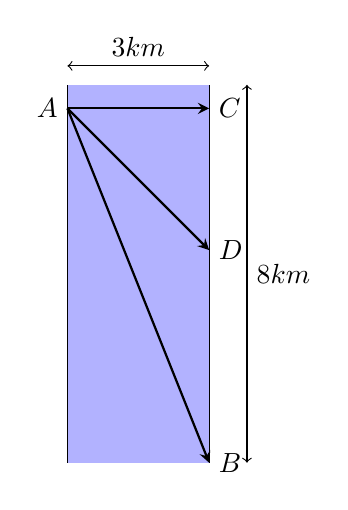
\begin{tikzpicture}[scale=0.6]
			% Vẽ dòng sông
			\fill[blue!30] (0,0) rectangle (3,8);
			\draw (0,0) -- (0,8);
			\draw (3,0) -- (3,8);
			\coordinate (A) at (0,7.5);
			\coordinate (C) at (3,7.5);
			\coordinate (B) at (3,0);
			\coordinate (D) at (3,4.5); % Điểm D giả định
			\draw[->, thick, >=stealth] (A) -- (C);
			\draw[->, thick, >=stealth] (A) -- (D);
			\draw[->, thick, >=stealth] (A) -- (B);
			\node[left] at (A) {$A$};
			\node[right] at (C) {$C$};
			\node[right] at (D) {$D$};
			\node[right] at (B) {$B$};
			\draw[<->] (0,8.4) -- (3,8.4) node[midway, above] {$3 \text{ km}$};
			\draw[<->] (3.8,8) -- (3.8,0) node[midway, right] {$8 \text{ km}$};
		\end{tikzpicture}
	}
	\shortans{$17$}
	\loigiai{
		Gọi $CD = x \text{ (km)} \Rightarrow DB = 8 - x \text{ (km)}$, điều kiện $0 \le x \le 8$.
		Khi đó ta có:
		\begin{itemize}
			\item $AD = \sqrt{3^2 + x^2} = \sqrt{x^2 + 9} \Rightarrow t_{AD} = \dfrac{\sqrt{x^2 + 9}}{6}$.
			\item $DB = 8 - x \Rightarrow t_{DB} = \dfrac{8 - x}{8}$.
		\end{itemize}
		$\Rightarrow t = t_{AD} + t_{DB} = \dfrac{\sqrt{x^2 + 9}}{6} + \dfrac{8 - x}{8} = f(x)$.
		Xét $f'(x) = \dfrac{x}{6\sqrt{x^2 + 9}} - \dfrac{1}{8}, f'(x) = 0 \Leftrightarrow x = \dfrac{9\sqrt{7}}{7}$.
		Lập bảng biến thiên của hàm số $f(x)$ với $0 \leq x \le 8$:
		\begin{center}
			
\begin{tikzpicture}
				\tkzTabInit[lgt=1.5, espcl=3]
				{$x$ /1, $f'(x)$ /1, $f(x)$ /2}
				{$0$, $\frac{9\sqrt{7}}{7}$, $8$}
				\tkzTabLine{, -, 0, +, }
				\tkzTabVar{+ / $\frac{3}{2}$, - / $\frac{8+\sqrt{7}}{8}$, + / $\frac{\sqrt{73}}{6}$}
			\end{tikzpicture}
		\end{center}
		Dựa vào bảng ta có $\min \limits_{[0;8]} = \dfrac{8 + \sqrt{7}}{8} = 1 + \dfrac{1}{8}\sqrt{7}$ \\
		Như vậy $a = 1, b = 1, c = 8, d = 7 \Rightarrow a + b + c + d = 1 + 1 + 8 + 7 = 17$.
	}
\end{ex}

\begin{ex}%[TT-BacNinh-ChuyenBacNinh-lan1]%[Dương Tấn Đạt, 26-2-DuAnDeTHPT2025-2026]%[1H8V7-4]
	Cho hình lăng trụ $ABC.A'B'C'$ có đáy là tam giác đều cạnh $2$. Hình chiếu vuông góc của $A'$ lên mặt phẳng $(ABC)$ trùng với trọng tâm tam giác $ABC$. Biết khoảng cách giữa hai đường thẳng $AA'$ và $BC$ bằng $\dfrac{\sqrt{3}}{2}$. Tính thể tích $V$ của khối lăng trụ $ABC.A'B'C'$ (kết quả làm tròn đến hàng phần trăm).
	\shortans{$1{,}15$}
	\loigiai{
		\begin{center}
			\resizebox{0.5\textwidth}{!}{
				\begin{tikzpicture}[scale=1.2, font=\footnotesize, line join=round, line cap=round, >=stealth]
					\path
					(0,0) coordinate (A)
					(4,0) coordinate (C)
					(1.5,-1.5) coordinate (B)
					;
					\coordinate (I) at ($(B)!0.5!(C)$);
					\coordinate (G) at ($(A)!2/3!(I)$);
					
					\coordinate (A') at ($(G)+(0,4)$);
					\coordinate (B') at ($(B)+(A')-(A)$);
					\coordinate (C') at ($(C)+(A')-(A)$);
					
					\coordinate (K) at ($(A)!0.4!(A')$);
					\coordinate (J) at ($(A)!2/3!(K)$);
					\draw[dashed] (A)--(C) (A')--(G) (G)--(I) (A)--(I) (G)--(J) (I)--(K);
					\draw (A)--(B) (B)--(C) (A)--(A') (B)--(B') (C)--(C') (A')--(B') (B')--(C') (C')--(A');
					\foreach \p/\q in {A/180, J/180, K/180, B/-90, I/-90, G/-135, C/0, C'/0, B'/-45, A'/90} {
						\fill[black] (\p) circle (1.0pt);
						\node[shift={(\q:3mm)}] at (\p) {$\p$};
					}
				\end{tikzpicture}
			}
		\end{center}
		Gọi $G$ là trọng tâm tam giác $ABC$, $I$ là trung điểm $BC$, $J$ là hình chiếu của $G$ lên $AA'$, $K$ là hình chiếu của $I$ lên $AA'$. \\
		Ta có: $AA' \parallel BB' \Rightarrow d(AA', BC) = d(AA', (BB'C'C)) = d(A, (BB'C'C))$. \\
		Vì $\Delta ABC$ đều nên $AI \perp BC$, mà $A'G \perp (ABC) \Rightarrow A'G \perp BC$
		$\Rightarrow BC \perp (AA'I) \Rightarrow IK \perp BC$, suy ra $IK = d(A, (BB'C'C)) = \dfrac{\sqrt{3}}{2}$. \\
		Xét tam giác $AIK$ có $JG \parallel IK \Rightarrow \dfrac{JG}{KI} = \dfrac{AG}{AI} = \dfrac{2}{3} \Rightarrow JG = \dfrac{\sqrt{3}}{3}$. \\
		Tam giác $ABC$ đều cạnh $2$ có $AI = \dfrac{2\sqrt{3}}{2} = \sqrt{3} \Rightarrow AG = \dfrac{2}{3}AI = \dfrac{2\sqrt{3}}{3}$. \\
		Xét tam giác vuông $AGA'$ có: $\dfrac{1}{JG^2} = \dfrac{1}{AG^2} + \dfrac{1}{A'G^2} \Rightarrow A'G = \dfrac{2}{3}$. \\
		Thể tích khối lăng trụ: $V_{ABC.A'B'C'} = A'G \cdot S_{ABC} = \dfrac{2}{3} \cdot \dfrac{2^2\sqrt{3}}{4} = \dfrac{2\sqrt{3}}{3} \approx 1{,}15$.
	}
\end{ex}

\Closesolutionfile{ans}
%  \indapan{3}{ans/ans-23-26-2-BacNinh-ChuyenBacNinh-L1}
